\documentclass[11pt,french]{book}
\input preambule_2013

\newcounter{exoc}
\newenvironment{exoc}[1]{%
  \refstepcounter{exoc}\textbf{Exercice \theexoc} :\hfill {\textbf{(#1)}}\par
  \medskip}%
{\medskip}

\pagestyle{empty}

\begin{document}

\begin{center}
\begin{tabularx}{\textwidth}{|>\centering m{2.5cm}|>\centering X|>{\centering\arraybackslash} m{2.5cm}|}
	\hline
		\seconde 7 &  Mardi 17 décembre \np{2013} & \textbf{\'Equations de droites} \\
	\hline
		\multicolumn{3}{|c|}{\bsc{Contrôle de mathématiques}} \\
	\hline
        \multicolumn{1}{|r}{\bsc{Nom}:} & \multicolumn{2}{l|}{} \\
		\multicolumn{1}{|r}{Prénom:} & \multicolumn{2}{l|}{} \\
	\hline
        \multicolumn{3}{|l|}{\bfseries Note et observations :} \\[1cm]
    \hline
\end{tabularx}\bigskip

{\itshape
Le barème est indicatif.\par
La rédaction est importante dans de nombreuses questions.\par
{\bfseries 2 points seront attribués à la qualité et la précision de la rédaction !}
}
\end{center}

\begin{exoc}{1 + 2 + 2 + 1 + 1 + 2 = 9 pts}
Dans cet exercice, on se place dans le repère orthonormé \OIJ ci-dessous. L'unité est le carreau.\medskip

\begin{minipage}{0.65\linewidth}
    \begin{enumerate}
        \item La droite $(d_1)$ passe par les points $A(1 \pv 1)$ et $B(3 \pv -5)$.
            \begin{enumerate}
                \item Placer les points $A$ et $B$ sur le repère et tracer la droite $(d_1)$.
                \item En détaillant précisément les calculs, déterminer l'équation réduite de la droite $(d_1)$.
            \end{enumerate}
        \item La droite $(d_2)$ a pour équation $y = 2x + 1$.
            \begin{enumerate}
                \item En détaillant précisément la démarche, tracer la droite $(d_2)$.
                \item Les droites $(d_1)$ et $(d_2)$ sont-elles parallèles ? Justifier la réponse en utilisant une propriété du cours.
                \item Les droites $(d_1)$ et $(d_2)$ sont-elles perpendiculaires ? Justifier précisément la réponse en utilisant une propriété du cours.
            \end{enumerate}
        \item On appelle $C$ le point d'intersection des droites $(d_1)$ et $(d_2)$. Calculer les coordonnées du point $C$. Donner les coordonnées sous forme fractionnaire.
    \end{enumerate}
\end{minipage}
\begin{minipage}{0.33\linewidth}
\begin{center}
    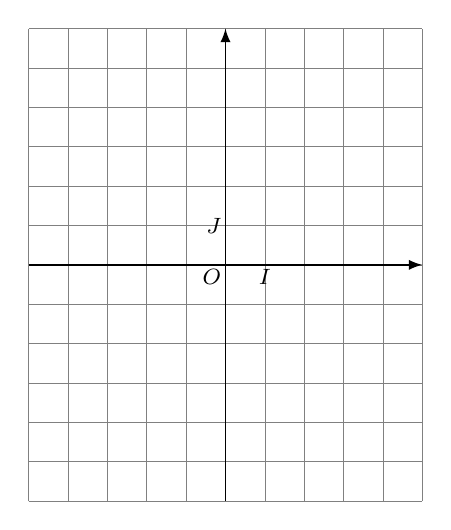
\begin{tikzpicture}[scale=0.5,>=latex]
        \def\xmin{-5}\def\xmax{5}\def\ymin{-6}\def\ymax{6}
        \draw[help lines] (\xmin,\ymin) grid (\xmax,\ymax);
        \draw[->,line width = 0.7pt] (\xmin,0) -- (\xmax,0);
        \draw[->,line width = 0.7pt] (0,\ymin) -- (0,\ymax);
        \draw (0,0) node[below left=-2pt] {\footnotesize $O$};
        \draw (1,0) node[below=-2pt] {\footnotesize $I$};
        \draw (0,1) node[left=-2pt] {\footnotesize $J$};
    \end{tikzpicture}
\end{center}
\end{minipage}
\end{exoc}\[*\]

\begin{exoc}{1 + 2 + 2 + 2 + 2 = 9 pts}
    Pour cet exercice, la figure \textbf{n'est pas} obligatoire.\par
    Dans un repère orthonormé \OIJ, on considère les points suivants définis par leurs coordonnées :
    \[R(1 \pv -2) \qq S(5 \pv 2) \qetq T(1\pv 5).\]

    \begin{enumerate}
        \item En expliquant la démarche, déterminer une équation de la droite $(RT)$.
        \item En détaillant précisément la démarche, déterminer l'équation réduite de la droite $(RS)$.
        \item On appelle $(\Delta)$ la droite parallèle à $(RS)$ passant par $T$.\par
        En détaillant précisément la démarche, déterminer l'équation réduite de la droite $(\Delta)$.
        \item Le point $U$ appartient à $(RS)$ et on sait que son ordonnée est $y_U = -4$.\par Calculer son abscisse $x_U$.
        \item Les points $T$, $O$ et $U$ sont-ils alignés ?
    \end{enumerate}

\end{exoc}

\end{document} 